\chapter{Nonlinear dynamics and chaos}
\label{ch:chaos}

\buildson{analytical mechanics (Chapter~\ref{ch:analytical})}

\chapterdek{When dead-simple rules turn impossible to predict --- and why the impossibility has a beautiful, universal structure of its own.}

\begin{prototype}
The logistic map, $x_{n+1} = r\,x_n(1 - x_n)$: a one-line model of a population that grows when small and starves when large. As the growth rate $r$ is turned up, the population settles down, then oscillates between two values, then four, then eight, and then --- with no randomness anywhere in the rule --- becomes chaotic. Its physical cousin is the double pendulum, whose tumbling no one can predict for more than a few swings.
\end{prototype}

Nearly every equation solved in an introductory course is linear. That is not because nature is linear; it is because linear equations are the ones we can solve. Superposition lets us break them into simple pieces (Chapter~\ref{ch:math}). Nonlinear equations offer no such mercy, and for centuries they were treated as hopeless special cases. In the last sixty years, aided by computers and geometric thinking, physicists and mathematicians discovered that nonlinear systems have a rich, beautiful, and in some ways universal behaviour --- including \emph{chaos}, deterministic behaviour so sensitive that it is unpredictable in practice.

\section{Flows on a line}

Start with the simplest dynamical system: one variable obeying $\dot x = f(x)$. There is no need to solve it. Plot $f(x)$; where $f>0$, $x$ increases, where $f<0$ it decreases. The \emph{fixed points}, where $f(x^*) = 0$, are equilibria. A fixed point is \emph{stable} if nearby points flow toward it, which happens when $f'(x^*) <0$; linearizing, a small deviation $\delta$ obeys $\dot\delta = f'(x^*)\,\delta$ and decays exponentially.

\begin{example}[Logistic growth]
A population with limited food obeys $\dot N = rN(1 - N/K)$. There are fixed points at $N=0$ (unstable: any population grows) and $N = K$, the carrying capacity (stable). Every positive population approaches $K$ along an S-shaped curve. In one dimension, that is all that can happen: trajectories move monotonically to fixed points or to infinity. No oscillation, no chaos.
\end{example}

\textbf{Bifurcations.} As a parameter changes, fixed points can appear, vanish, or exchange stability. These qualitative changes are called \emph{bifurcations}, and there are only a few basic kinds.
\begin{itemize}[itemsep=3pt]
  \item \textbf{Saddle-node}: $\dot x = r + x^2$. For $r<0$ there are two fixed points, one stable and one unstable; at $r = 0$ they collide and annihilate; for $r>0$ there are none, and $x$ runs away. This is how a system can lose its equilibrium suddenly --- how a slowly pushed object suddenly starts to slide, or a lake suddenly turns murky.
  \item \textbf{Pitchfork}: $\dot x = rx - x^3$. For $r<0$ the only fixed point is $x = 0$, stable. For $r>0$ it becomes unstable and two new stable fixed points appear at $\pm\sqrt r$. The system must choose one, breaking the symmetry $x\to-x$ of the equation. The bead on a spinning hoop (Problem~\ref{prob:bead-hoop}), the buckling of a column, a ferromagnet below its Curie temperature (Chapter~\ref{ch:statmech}), and the Higgs field (Chapter~\ref{ch:particle}) all do this.
\end{itemize}
Saddle-node bifurcations come with \emph{hysteresis}: turn the parameter back, and the system does not retrace its path. Many sudden transitions in climate, ecosystems, and engineering are of this type (Chapter~\ref{ch:geo}).

\section{Flows in the plane}

With two variables, $\dot x = f(x,y)$, $\dot y = g(x,y)$, much more can happen. Near a fixed point, linearize: $(\delta\dot x,\delta\dot y) = J\,(\delta x,\delta y)$ with $J$ the \emph{Jacobian} matrix of partial derivatives. Its eigenvalues (Chapter~\ref{ch:math}) classify the fixed point:
\begin{itemize}[itemsep=3pt]
  \item both real and negative: a stable \emph{node};
  \item real with opposite signs: a \emph{saddle}, attracting along one direction and repelling along another;
  \item complex with negative real part: a stable \emph{spiral} --- the damped oscillator of Chapter~\ref{ch:sho};
  \item purely imaginary: a \emph{centre}, surrounded by closed orbits --- the frictionless oscillator.
\end{itemize}

\begin{example}[The nonlinear pendulum]
The pendulum $\ddot\theta = -(g/\ell)\sin\theta$, written as a flow in $(\theta,\dot\theta)$, has centres at $\theta = 0,\pm2\pi,\dots$ (hanging down) and saddles at $\theta=\pm\pi$ (balanced upright). Small swings circle the centres; large enough energy carries the pendulum over the top, rotating forever. The two kinds of motion are separated by the \emph{separatrix}, the trajectory that creeps toward the upright position and takes infinitely long to arrive. The whole phase portrait can be drawn from the energy alone, without solving anything.
\end{example}

A genuinely new behaviour appears in two dimensions: the \textbf{limit cycle}, an isolated closed orbit that nearby trajectories spiral toward. A limit cycle is a self-sustained oscillation whose amplitude is set by the system itself, not by initial conditions. The van der Pol oscillator, $\ddot x - \mu(1-x^2)\dot x + x = 0$, has negative damping for small $x$ (pumping energy in) and positive damping for large $x$ (draining it), and settles onto one. Heartbeats, the squeal of a violin string, the flashing of a firefly, and the ticking of a pendulum clock's escapement are limit cycles. A stable fixed point can give birth to a limit cycle as a parameter changes; this is a \emph{Hopf bifurcation}, and it is how a steady flow past a cylinder begins to shed vortices rhythmically (Chapter~\ref{ch:fluids}).

But in two dimensions, chaos is impossible.

\begin{theorem}[Poincar\'e--Bendixson]
A bounded trajectory of a smooth autonomous flow in the plane approaches either a fixed point, or a closed orbit, or a cycle of fixed points connected by trajectories.
\end{theorem}
Trajectories cannot cross, and in a plane a curve that cannot cross itself has little room to misbehave. Chaos needs a third dimension.

\section{Chaos}

In 1963 the meteorologist Edward Lorenz simplified a model of convection in the atmosphere down to three equations:
\[
  \dot x = \sigma(y-x),\qquad \dot y = x(\rho - z) - y,\qquad \dot z = xy - \beta z,
\]
with $\sigma = 10$, $\beta = 8/3$, $\rho = 28$. Running it on an early computer, he restarted a calculation from numbers printed to three decimal places instead of six. Within a few simulated months the two runs had nothing to do with each other.

\begin{center}
\begin{tikzpicture}
  \node[inner sep=0] (img) at (0,0) {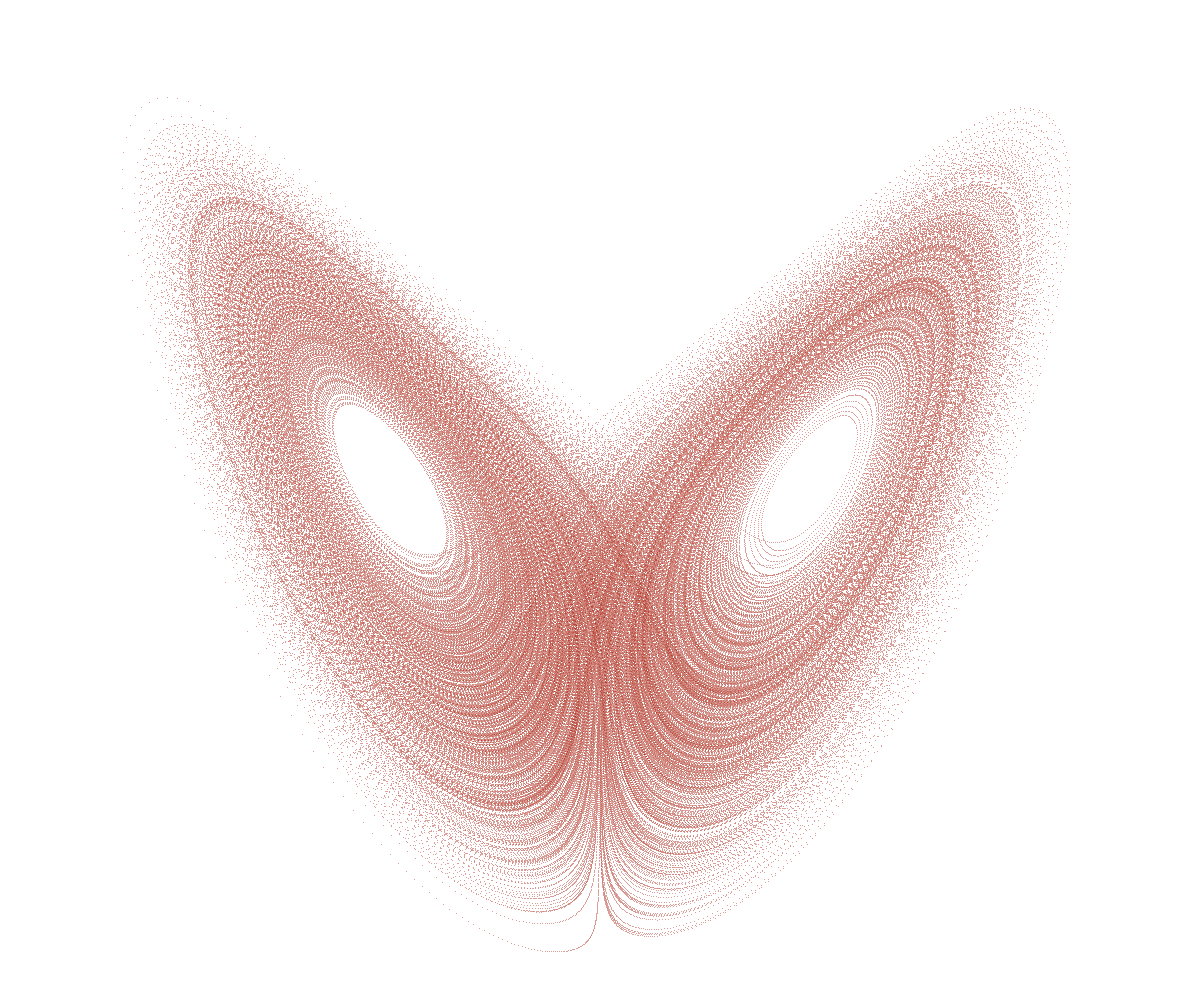
\includegraphics[width=0.55\linewidth]{figures/lorenz.png}};
  \node[font=\small,anchor=north] at (img.south) {The Lorenz attractor, projected onto the $(x,z)$ plane.};
\end{tikzpicture}
\end{center}

This is the defining feature of chaos: \textbf{sensitive dependence on initial conditions}. Two trajectories starting a distance $\delta_0$ apart separate exponentially,
\[
  \delta(t)\approx\delta_0\,e^{\lambda t},
\]
where $\lambda>0$ is the \emph{Lyapunov exponent}. Any uncertainty in the initial state, however small, grows until it is as large as the system itself, after a \emph{predictability horizon}
\[
  t_{\text{pred}}\approx\frac{1}{\lambda}\ln\frac{L}{\delta_0}.
\]
The logarithm is cruel: making measurements a thousand times more precise buys only $\ln1000\approx7$ more Lyapunov times. For the atmosphere, $1/\lambda$ is a day or two, so detailed weather forecasts are limited to about two weeks no matter how good our computers become. Lorenz called it the \emph{butterfly effect}.

Yet the motion is not random. The Lorenz trajectory never settles down and never repeats, but it stays forever on a butterfly-shaped set called a \textbf{strange attractor}. Volumes in its phase space shrink (the system is dissipative), so trajectories are squeezed onto a set of zero volume; but nearby trajectories also separate, so the set must be endlessly stretched and folded, like dough being kneaded. The result is a \emph{fractal}, with dimension about $2.06$: more than a surface, less than a solid.

\begin{keyidea}
Determinism does not imply predictability. A system can be governed by perfectly definite laws, with no randomness anywhere, and still be unpredictable in practice, because it amplifies every uncertainty exponentially. Chaos is how deterministic physics manufactures apparent randomness.
\end{keyidea}

\section{Maps, and the road to chaos}

Many questions about flows reduce to iterated \emph{maps} $x_{n+1} = F(x_n)$, for example by recording a trajectory once per orbit. The logistic map is the simplest that shows everything.
\begin{itemize}[itemsep=3pt]
  \item For $1<r<3$, $x_n$ converges to the fixed point $x^* = 1 - 1/r$.
  \item At $r=3$ the fixed point loses stability (the slope of the map there passes through $-1$), and a stable cycle of period $2$ appears.
  \item At $r \approx 3.449$ the 2-cycle gives way to a 4-cycle, then an 8-cycle at $3.544$, a 16-cycle at $3.564$, and so on, the intervals shrinking geometrically.
  \item At $r_\infty\approx3.5699$ the period becomes infinite: chaos. Beyond it, chaotic bands are interrupted by \emph{windows} of periodic behaviour, the largest a period-3 window near $r = 3.83$.
\end{itemize}

\begin{center}
\begin{tikzpicture}
  \node[anchor=south west,inner sep=0] (img) at (0,0) {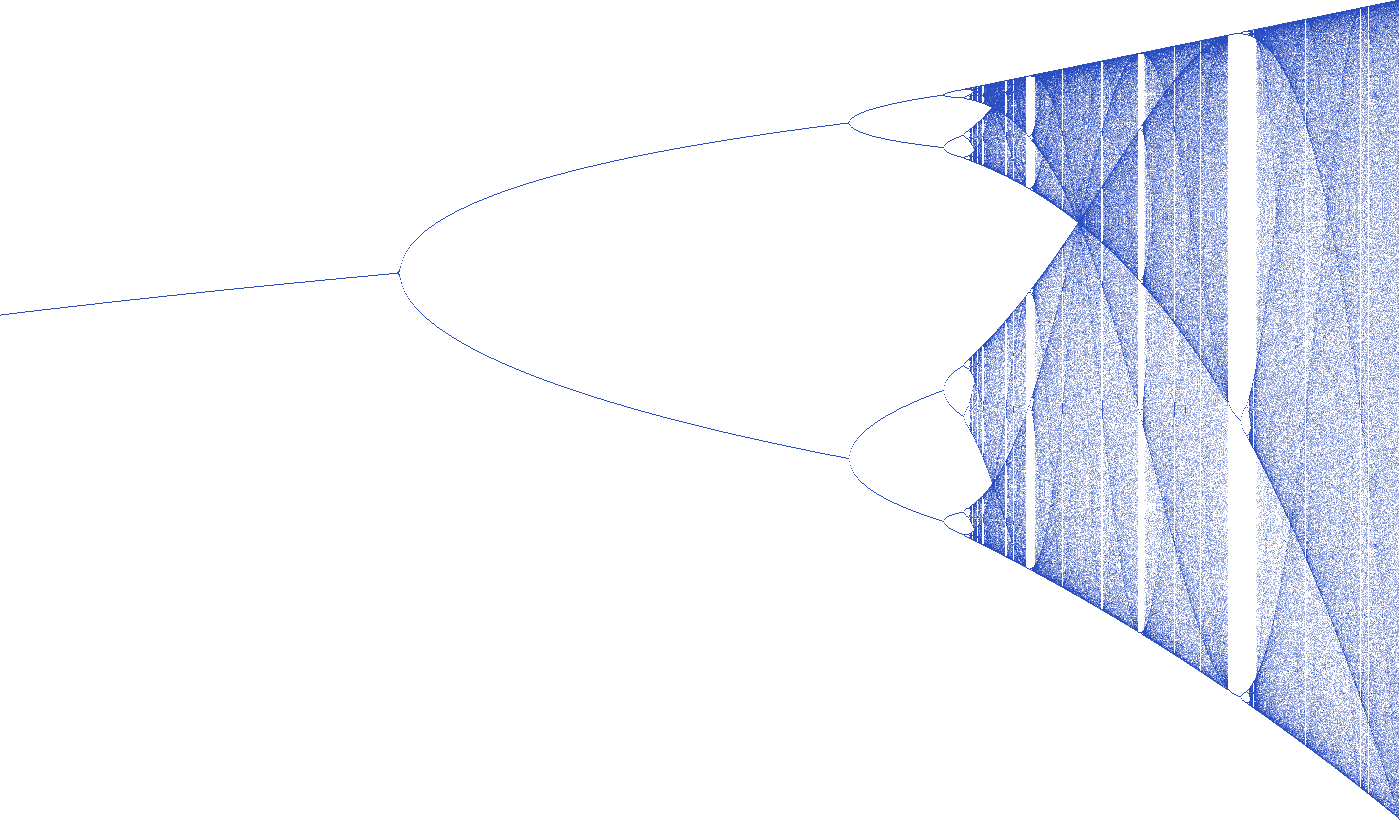
\includegraphics[width=0.82\linewidth]{figures/logistic-bifurcation.png}};
  \begin{scope}[x={(img.south east)},y={(img.north west)}]
    \draw[-{Stealth[length=5pt]}] (0,0) -- (1.04,0) node[right] {$r$};
    \draw[-{Stealth[length=5pt]}] (0,0) -- (0,1.07) node[above] {$x$};
    \foreach \t/\lab in {0/2.6, 0.2857/3.0, 0.6429/3.5, 1/4.0}
      \draw (\t,0) -- (\t,-0.02) node[below,font=\small] {\lab};
    \foreach \t/\lab in {0/0, 0.5/0.5, 1/1}
      \draw (0,\t) -- (-0.012,\t) node[left,font=\small] {\lab};
  \end{scope}
\end{tikzpicture}

{\small The long-run values of the logistic map as the parameter $r$ increases: period doubling, then chaos.}
\end{center}

In 1975 Mitchell Feigenbaum, playing with a pocket calculator, noticed that the ratios of successive intervals between period doublings converge to a constant,
\[
  \delta = \lim_{n\to\infty}\frac{r_n - r_{n-1}}{r_{n+1}-r_n} = 4.6692\ldots
\]
and then discovered that the \emph{same} constant appears for every map with a single smooth hump, not just the logistic map. It has since been measured in convecting fluids, dripping taps, electronic circuits, and lasers. This \textbf{universality} is the same phenomenon as in critical phenomena (Chapter~\ref{ch:statmech}), explained by the same renormalization ideas: near the onset of chaos, the details of the system wash out.

\section{Hamiltonian chaos}

Systems without friction cannot have attractors, because Liouville's theorem forbids phase-space volumes from shrinking (Chapter~\ref{ch:analytical}). They can still be chaotic. Poincar\'e discovered this in 1890 while studying the \emph{three-body problem} --- the motion of three masses under gravity --- for a prize offered by the King of Sweden. He found that the problem could not be solved in closed form, because some trajectories tangle with each other in unimaginably complicated ways. His prize essay contained a mistake, and fixing it gave birth to chaos theory.

For nearly integrable systems, the \textbf{KAM theorem} (Kolmogorov, Arnold, Moser) says most regular orbits survive small perturbations, but chaotic regions grow between them as the perturbation increases. The solar system is a case in point: it is chaotic, with a Lyapunov time of about five million years for the inner planets. We cannot predict where the Earth will be in its orbit a hundred million years from now, though the orbit itself is very likely stable for billions of years. Saturn's moon Hyperion tumbles chaotically, and the gaps in the asteroid belt are where chaos has cleared the orbits out.

\section{Fractals}

A \emph{fractal} is a shape with structure at every scale. Its \emph{dimension} can be found by counting how many boxes of size $\epsilon$ it takes to cover it: if $N(\epsilon)\propto\epsilon^{-D}$, the dimension is $D$. A line has $D = 1$ and a filled square $D = 2$, but the \emph{Cantor set} --- remove the middle third of a segment, then the middle thirds of what remains, forever --- has $D = \ln2/\ln3\approx0.63$. Coastlines, clouds, river networks, lungs, and the boundaries of chaotic regions are approximately fractal, and Mandelbrot's question ``How long is the coast of Britain?'' has the answer that it depends on your ruler.

\section{Solitons and patterns}

Nonlinearity does not only destroy order; it can create it. In 1834 the engineer John Scott Russell followed, on horseback, a single hump of water that a stopped barge had sent rolling along a canal; it travelled for miles without changing shape. Ordinarily, dispersion would spread such a pulse out (Chapter~\ref{ch:waves}), and nonlinearity would steepen it into a breaking wave. In a \emph{soliton} the two effects exactly balance. Solitons appear in optical fibres, where they carry pulses without distortion, in plasmas, and in quantum field theory.

Nonlinear systems driven away from equilibrium also form spontaneous \emph{patterns}: the hexagonal convection cells in a pan of heated oil, the stripes of a zebra (which Turing proposed in 1952 arise from chemicals that react and diffuse at different rates), the spirals of certain chemical reactions, and the regular ripples of sand dunes.

\section{Synchronization}

In 1665 Christiaan Huygens, ill in bed, noticed that two pendulum clocks hanging from the same beam always ended up swinging in exact opposition, however he started them. Weakly coupled oscillators with nearby frequencies tend to \emph{lock} together. Thousands of fireflies in Southeast Asian trees flash in unison; pacemaker cells in the heart fire together; audiences clapping fall into rhythm; and the Moon's rotation is locked to its orbit. In the \emph{Kuramoto model}, many oscillators with a spread of natural frequencies couple to their average, and above a critical coupling strength a synchronized group spontaneously forms --- a phase transition in time.

\section{Problems}

\begin{problems}
\prob{1}\core Find the fixed points of $\dot x = x - x^3$ and determine their stability. Sketch $x(t)$ for several initial conditions. Which of these behaviours could a linear equation produce?

\prob{1} For $\dot x = r + x^2$, find the fixed points as a function of $r$, determine their stability, and draw the bifurcation diagram. For $r$ slightly positive, show that $x$ spends a long time near $x = 0$ (a ``bottleneck''), and estimate how long, using $\int\dd x/(r+x^2)$.

\prob{1} Classify the fixed point at the origin of $\dot x = y$, $\dot y = -x - 0.2y$. What physical system is this?

\prob{2}\core For the logistic map, find the fixed points and show that $x^* = 1-1/r$ is stable for $1<r<3$. Then find the period-2 orbit for $r>3$ by solving $F(F(x)) = x$ (factor out the fixed points), and show that it is stable for $3<r<1+\sqrt6\approx3.449$.

\prob{2} The doubling map $x_{n+1} = 2x_n \bmod 1$ shifts the binary expansion of $x$ one place left at each step. Show that its Lyapunov exponent is $\ln 2$, and interpret this: each iteration, one more binary digit of the initial condition becomes visible in the motion. Why does this make long-term prediction hopeless?

\prob{2} Weather forecasts have a Lyapunov time of roughly $1.5$ days. Initial measurements are accurate to about one part in $10^{5}$ of the relevant scale. Estimate the predictability horizon. By how much would it improve if measurements became a thousand times better?

\prob{2} Draw the phase portrait of the frictionless pendulum using energy conservation. Find the energy of the separatrix, and show that the period of a pendulum whose amplitude approaches $\pi$ diverges logarithmically.

\prob{2} For the Lorenz equations, show that the origin is a stable fixed point for $\rho<1$. For $\rho>1$, show that two more fixed points appear at $x = y = \pm\sqrt{\beta(\rho-1)}$, $z = \rho-1$. (These are the centres of the two ``wings.'')

\prob{2} Find the fractal dimension of the Cantor set, and of the Koch snowflake curve (in which each segment is replaced by four segments one third as long). Show that the Koch snowflake has infinite perimeter but finite area.

\prob{3}\core Explain, using the Poincar\'e--Bendixson theorem, why a pendulum with friction cannot be chaotic, but a pendulum with friction that is also driven by a periodic torque can be. (What is the dimension of the driven pendulum's phase space?) How many dimensions does a discrete map need to be chaotic?

\prob{3} \emph{(Phase locking.)} Two oscillators with natural frequencies $\omega_1$ and $\omega_2$ are coupled: $\dot\theta_1 = \omega_1 + K\sin(\theta_2-\theta_1)$, $\dot\theta_2 = \omega_2 + K\sin(\theta_1 - \theta_2)$. Write an equation for the phase difference $\phi = \theta_1 - \theta_2$ and show that the oscillators lock (with $\phi$ constant) if and only if $\abs{\omega_1-\omega_2}\le2K$. What happens just outside this range?

\prob{3} \emph{(Feigenbaum's constant by hand.)} The first period-doubling points of the logistic map are $r_1 = 3$, $r_2 = 1+\sqrt6\approx3.4495$, $r_3\approx3.5441$, $r_4\approx3.5644$. Compute the ratios of successive intervals and compare with $\delta = 4.669$. Assuming the intervals shrink geometrically by exactly $\delta$, predict the accumulation point $r_\infty$ and compare with $3.5699$. Then explain why the same $\delta$ appears in the dripping of a tap.
\end{problems}

\begin{reading}
\rd{Steven H.\ Strogatz, \emph{Nonlinear Dynamics and Chaos}}{The best introduction by far: geometric, physical, applied, and fun. This chapter follows its outline.}
\rd{James Gleick, \emph{Chaos: Making a New Science}}{The popular history of how chaos was discovered.}
\rd{Edward Ott, \emph{Chaos in Dynamical Systems}}{A more advanced and complete treatment.}
\rd{Cvitanovi\'c et al., \emph{Chaos: Classical and Quantum} (ChaosBook.org)}{A free online book that goes very deep, including periodic orbit theory and quantum chaos.}
\end{reading}
